\documentclass[12pt,aspectratio=169]{beamer}

\usetheme{default}
\usepackage{slidetemplate}

\usepackage{tikz}
\usetikzlibrary{arrows}

\usepackage{hyperref}
\usepackage{biblatex}
\addbibresource{references.bib}

\hypersetup{allcolors=amaranth}
  
\title{Federated Reinforcement Learning}
\author{Paul Mangold, École Polytechnique}
\conf{REDEEM Retreat @ Annecy, September 24th 2025}

\begin{document}

\begin{frame}
  \titlepage
\end{frame}

\begin{frame}{Refresher on Reinforcement Learning}


  \begin{minipage}[t]{0.45\linewidth}
    \vspace{-2em}
    In RL, agent:
    \begin{itemize}
    \item take actions in an environment
    \item collect reward after their action
    \item learn to obtain better rewards
    \end{itemize}
  \end{minipage}\hspace{2em}
  \begin{minipage}[t]{0.45\linewidth}
    
    \includegraphics[width=0.5\linewidth]{images/ataribench.png}~~~~~%
    \includegraphics[width=0.45\linewidth]{images/maze_simple.pdf}

    \vspace{1em}
    
    \includegraphics[width=0.5\linewidth]{images/rlhf.jpeg}~~~~~~
    \includegraphics[width=0.45\linewidth]{images/Types_V2X.png}
  \end{minipage}
  
\end{frame}

\begin{frame}{Refresher on Reinforcement Learning}

  \vspace{2.5em}
  
  \begin{minipage}{0.65\linewidth}
    Environment:
    \begin{itemize}
      \small
    \item set of states $\mathcal{S}$
    \item set of actions $\mathcal{A}$
    \item rewards, typically in $[0, 1]$
    \item transition $P(\cdot|s,a)$ for $s, a \in \mathcal{S} \times \mathcal{A}$
    \end{itemize}


    \vspace{0.5em}
    
    % Agent:
    % \begin{itemize}
    %   \small
    % \item is in a state $s \in \mathcal{S}$
    % \item acts according to a policy $a \sim \pi(\cdot | s)$
    % \item reaches a new state $s' \sim P(\cdot | s, a)$
    % \item receives a reward $r(s,a)$
    % \end{itemize}

  \end{minipage} \hspace{-5em}%
  \begin{minipage}{0.3\linewidth}
    \resizebox{1.8\linewidth}{!}{
      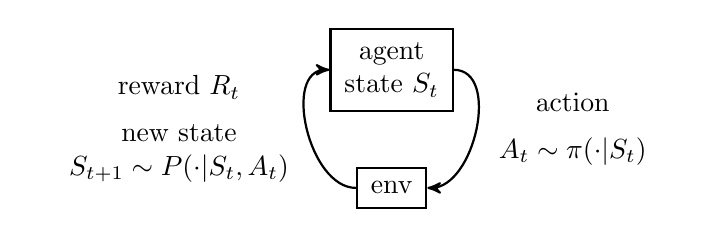
\begin{tikzpicture}[->,>=stealth',auto,node distance=3cm,
        thick,main node/.style={circle,draw,font=\sffamily\Large\bfseries}]
        % nodes 
        \node[draw,fill=white, align=center, inner sep=5pt] (A1) at (0, 1.5) {agent \\ state $S_t$};
        \node[draw, fill=white, align=center, inner sep=5pt] (B1) at (0, 0) {env};

        % arrows
        \draw [->] (B1.west) to [out=180,in=180] (A1.west) ;
        \draw [->] (A1.east) to [out=0,in=0] (B1.east);

        \node[align=center,inner sep=15pt] (A1t) at (-2.7, 0.75) {reward $R_t$ \\[0.5em] new state \\ $S_{t+1} \sim P(\cdot | S_t, A_t)$};
        \node[align=center,inner sep=15pt] (B1t) at (2.3, 0.75) {action \\[0.5em] $A_t \sim \pi(\cdot | S_t)$};
%        \node[align=center,inner sep=15pt] (C1t) at (3.5, 0.75) {\includegraphics[width=4em]{images/sedan-car-icon.pdf}};

      \end{tikzpicture}
    }
  \end{minipage}

  \begin{center} \large
    \textbf{\textcolor{amaranth}{Goal:}} learn $\pi$ to get good rewards
  \end{center}

\end{frame}


\begin{frame}{Example: CartPole}
  \qquad
  \begin{minipage}[t]{0.3\linewidth}
    
  \begin{figure}
    \centering
    \includegraphics[width=\linewidth]{images/cart-pole.png}
    \label{fig:enter-label}
  \end{figure}

  \end{minipage}\qquad\quad
  \begin{minipage}[t]{0.5\linewidth}

    \vspace{3em}

    Goal: keep the stick up

    \begin{itemize}
    \item state: angle of the stick
    \item reward: $1$ if still up, $0$ otherwise
    \end{itemize}

    \vspace{1em}

    Idea: run episodes of length $H = 250$

    $\rightarrow$ adapt policy after each episode

  \end{minipage}
  
\end{frame}

\begin{frame}{Example: CartPole}
  Cumulative reward, 1 cart

  \vspace{-1em}
  
  \begin{figure}
    \centering
    \resizebox{!}{9em}{
    \begin{tikzpicture}
      \node at (0, 0)  {~};
      \node at (0, 2)  {\includegraphics[width=0.05\linewidth]{images/cart-pole.png}};
      \node at (0, 4)  {~};
    \end{tikzpicture}}
    \includegraphics[width=0.35\linewidth]{images/CartPole1.png}

    \label{fig:enter-label}
  \end{figure}

\end{frame}

\begin{frame}[t]{Two Big Questions in Reinforcement Learning}
  \begin{enumerate}
  \item \textbf{\textcolor{amaranth}{Policy evaluation}}: evaluate if a policy is good

    \vspace{1em}
    
    \only<2>{
      take a policy $\pi$

      goal: approximate the expected sum of reward for each $s \in \mathcal{S}$
      \begin{align*}
        V^\pi(s) = \mathbb{E}\Big[ \sum_{t=0}^\infty \gamma^t R(S_t, A_t) | S_0 = s\Big]
      \end{align*}

      where $A_{t} \sim \pi(\cdot|S_t)$ and $S_{t+1} \sim P(\cdot| S_t, A_t)$

      \vspace{2em}
    }
 
  \item \textbf{\textcolor{amaranth}{Policy optimization}}: find a good policy

    \vspace{1em}
    
    \only<3>{
      find the best policy (according to value), for all $s \in \mathcal{S}$
      \begin{align*}
        \pi_\star(\cdot|s) \in \arg\max_{\pi} V^{\pi}(s)
      \end{align*}
    }
  \end{enumerate}
  
\end{frame}

\begin{frame}{1. Policy Evaluation: TD Learning}

  \pause
  
  State Value function:
  \begin{align*}
    \nonumber 
    V^{(\pi)}(s) = \mathbb{E}\left[
    \sum_{t=0}^\infty \gamma^t R(S_{t},A_{t})
    ~\bigg|~ {S_{0}=s}
    \right]
  \end{align*}


  \pause

  Expanding the first step, we obtain the Bellman equation:
  \begin{align*}
    V^{(\pi)}(s)
    & =
    \mathbb{E}[ R(s, A_0) ]
    +
    \gamma
    \sum_{a \in \mathcal{A}}
    \pi(a | s)
    \mathbb{E} \left[
    \sum_{t=1}^\infty  \gamma^{t-1} R(S_t, A_t)
    \right]
    \\
    & = 
    \mathbb{E}[ R(s, A_0) ]
      +
    \gamma
    \sum_{a \in \mathcal{A}}
      \pi(a | s)
      \sum_{s' \in \mathcal{S}}
      P(s' | s, a)
      V^{(\pi)}(s')
  \end{align*}

\end{frame}

\begin{frame}{1. Policy Evaluation: TD Learning}
  The function $V^{(\pi)}$ satisfies the Bellman equation
  \begin{align}
    \label{eq:fixed-td}     \tag{$\star$}
    V^{(\pi)} - R - \gamma P V^{(\pi)} = 0
  \end{align}

  \pause

  Temporal difference learning finds $V^{(\pi)}$ by solving this equation: 
  \begin{itemize}
  \item take action $A_t \sim \pi(\cdot|S_t)$
  \item receive reward $R(S_t, A_t)$ and $S_{t+1} \sim P(\cdot|S_t, A_t)$
  \item update the current estimate $\hat{V}_t^{(\pi)}$ with the error from \eqref{eq:fixed-td}
    \begin{align*}
      \hat{V}_{t+1}^{(\pi)}(S_t) = \hat{V}_t^{(\pi)}(S_t) - \alpha ( V_t^{(\pi)}(S_t) - R(S_t, A_t) + \gamma P V_t^{(\pi)}(S_t)  )
    \end{align*}
  \end{itemize}

  \textcolor{amaranth}{$\boldsymbol{\Rightarrow}$}
  eventually, $\hat{V}_t^{(\pi)}$ converges to $ V^{(\pi)}$
  
\end{frame}

% \begin{frame}{From Value to Bellman}
%   The functions $V^\star$ and $Q^\star$ for \textcolor{amaranth}{\bfseries the best policy $\mathbf{\pi^\star}$} satisfy
%   \begin{align*}
%     Q_h^{(\pi^\star)}(s,a) & =  r_h(s,a) + P_h V_{h+1}^{(\pi^\star)} (s,a) \\ 
%     V_{h+1}^{(\pi^\star)} (s) &= \max Q_h^{(\pi^\star)} (s,  a)
%   \end{align*}

%   \vspace{1em}

%   We can thus learn $\pi^\star$ by iterating these equations!

%   \textcolor{amaranth}{\bfseries
%     $\rightarrow$ Problem: the transition kernels $P_h$ are unknown!
%   }


% \end{frame}

\begin{frame}{2. Policy Optimization: Policy Gradient Method}

  \pause
  
  The value function is
  \begin{align*}
    V^{(\pi)}(s)
    & =
      \mathbb{E}\left[
      \sum_{t=0}^\infty \gamma^t R(S_{t},A_{t})
      ~\bigg|~ {S_{0}=s}
      \right]
    \\
    & =
      \sum_{t=0}^\infty
      \gamma^t
      \sum_{s \in \mathcal{S}} \sum_{a \in \mathcal{A}}
      \mathbb{P}(S_t = s, A_t = a)
      \mathbb{E}[R(S_{t},A_{t})]
  \end{align*}

  Parameterize the policy $\pi_\theta$ by $\theta \in \mathbb{R}^{SA}$, and update
  \begin{align*}
    \theta_{t+1}
    & =
      \theta_t
      + \alpha \nabla_\theta V^{(\pi_\theta)}
  \end{align*}

  \textcolor{amaranth}{$\boldsymbol{\Rightarrow}$} the policy $\pi_{\theta_t}$ converges to an optimal policy $\pi_{\star}$
\end{frame}

\begin{frame}{The problem of Reinforcement Learning:}
  \begin{center}
    \Large
    All these methods require \textbf{a lot} of samples to converge
    
    \includegraphics[width=\textwidth]{images/millionsamples.png}
  \end{center}

  from \fullcite{schulman2017proximal}
  
\end{frame}

\begin{frame}

  \begin{center}
    \textcolor{amaranth}{
      \huge   {Federated Reinforcement Learning}
    }
  \end{center}
\end{frame}

\begin{frame}{Federated Reinforcement Learning}

  Idea: collaborate to solve these problems together \textbf{faster}

  \begin{center}
  \resizebox{!}{14em}{
      \begin{tikzpicture}[->,>=stealth',auto,node distance=3cm,
        thick,main node/.style={circle,draw,font=\sffamily\Large\bfseries}]
        % nodes 
        \node[draw,fill=white, align=center, inner sep=5pt] (A1) at (0, 1.5) {agent 1 \\ $s_t^{(1)}$};
        \node[draw, fill=white, align=center, inner sep=5pt] (B1) at (0, 0) {env 1};

        
        \node[draw,fill=white, align=center, inner sep=5pt] (A2) at (0, -1.5) {agent 2 \\ $s_t^{(2)}$};
        \node[draw, fill=white, align=center, inner sep=5pt] (B2) at (0, -3) {env 2};

        \node (dots) at (0, -4) {$\cdots$};
        
        \node[draw,fill=white, align=center, inner sep=5pt] (An) at (0, -5.5) {agent n \\ $s_t^{(n)}$};
        \node[draw, fill=white, align=center, inner sep=5pt] (Bn) at (0, -7) {env n};


        % arrows
        \draw [->] (B1.west) to [out=180,in=180] (A1.west) ;
        \draw [->] (A1.east) to [out=0,in=0] (B1.east);
        \draw [->] (B2.west) to [out=180,in=180] (A2.west) ;
        \draw [->] (A2.east) to [out=0,in=0] (B2.east);
        \draw [->] (Bn.west) to [out=180,in=180] (An.west) ;
        \draw [->] (An.east) to [out=0,in=0] (Bn.east);

        \node[align=center,inner sep=15pt] (A1t) at (-1.7, 0.75) {$r_t^{(1)}$ \\[0.5em] $S_{t+1}^{(1)}$};
        \node[align=center,inner sep=15pt] (B1t) at (1.8, 0.75) {$a_t^{(1)}$};
        \node[align=center,inner sep=15pt] (C1t) at (-4, 0.75) {\includegraphics[width=4em]{images/sedan-car-icon.pdf}};

        \node[align=center,inner sep=15pt] (A2t) at (-1.7, -2.25) {$r_t^{(2)}$ \\[0.5em] $S_{t+1}^{(2)}$};
        \node[align=center,inner sep=15pt] (B2t) at (1.8, -2.25) {$a_t^{(2)}$};

        \node[align=center,inner sep=15pt] (C2t) at (-4, -2.25) {\includegraphics[width=4em]{images/logistic-van-icon.pdf}};


        \node[align=center,inner sep=15pt] (Ant) at (-1.7, -6.25) {$r_t^{(n)}$ \\[0.5em] $S_{t+1}^{(n)}$};
        \node[align=center,inner sep=15pt] (Bnt) at (1.8, -6.25) {$a_t^{(n)}$};

        \node[align=center,inner sep=15pt] (Cnt) at (-4, -6.25)  {\includegraphics[width=4em]{images/suv-car-icon.pdf}};

        \node[fill=white, align=center, inner sep=5pt] (model) at (12, -2.7) {global policy};

        \node[draw, fill=white, align=center, inner sep=24pt] (algo) at (7, -2.7) {central server};
        % arrows
        \draw[<->] (B1t) to (algo);
        \draw[<->] (B2t) to (algo);
        \draw[<->] (Bnt) to (algo);
        \draw[->] (algo) to (model);

      \end{tikzpicture}   

    }
    
  \end{center}

\end{frame}

\begin{frame}{Example: CartPole}
  Cumulative reward, 1 cart vs. 10 carts

  \vspace{-1em}
  
  \begin{figure}
    \centering
    \resizebox{!}{9em}{
    \begin{tikzpicture}
      \node at (0, 0)  {~};
      \node at (0, 2)  {\includegraphics[width=0.05\linewidth]{images/cart-pole.png}};
      \node at (0, 4)  {~};
    \end{tikzpicture}}
    \includegraphics[width=0.35\linewidth]{images/CartPole1.png}
    \qquad
    \resizebox{!}{9em}{
    \begin{tikzpicture}
      \node at (0, 0)  {\includegraphics[width=0.05\linewidth]{images/cart-pole.png}};
      \node at (0, 1)  {\includegraphics[width=0.05\linewidth]{images/cart-pole.png}};
      \node at (0, 2)  {\includegraphics[width=0.05\linewidth]{images/cart-pole.png}};
      \node at (0, 3)  {\includegraphics[width=0.05\linewidth]{images/cart-pole.png}};
      \node at (0, 4)  {\includegraphics[width=0.05\linewidth]{images/cart-pole.png}};
      \node at (1, 0)  {\includegraphics[width=0.05\linewidth]{images/cart-pole.png}};
      \node at (1, 1)  {\includegraphics[width=0.05\linewidth]{images/cart-pole.png}};
      \node at (1, 2)  {\includegraphics[width=0.05\linewidth]{images/cart-pole.png}};
      \node at (1, 3)  {\includegraphics[width=0.05\linewidth]{images/cart-pole.png}};
      \node at (1, 4)  {\includegraphics[width=0.05\linewidth]{images/cart-pole.png}};
    \end{tikzpicture}}
    \includegraphics[width=0.35\linewidth]{images/CartPole10.png}
    \label{fig:enter-label}
  \end{figure}

\end{frame}


\begin{frame}
  \begin{center}
    \textcolor{amaranth}{
      \huge Question: \\[1em]
      \LARGE How does RL benefit from federated learning?
    }

    \vspace{2em}

    \pause

  \begin{itemize} \Large
  \item[$\rightarrow$] Can it accelerate the training?
  \item[$\rightarrow$] How to handle heterogeneity?
  \item[$\rightarrow$] How to reduce communications?
  \end{itemize}
  \end{center}

\end{frame}


\begin{frame}{Heterogeneity in Reinforcement Learning}

  Take $N$ agents with transition kernels $P^{(c)}$ and rewards $r^{(c)}$

  Two types of heterogeneity, for $c \neq c' \in \{1, \dots, N\}$
  \begin{itemize}
  \item[$\rightarrow$] transition kernel heterogeneity:
    \begin{center}
      for $s, a, s' \in \mathcal{S} \times \mathcal{A} \times \mathcal{S}$,
      $P^{(c)}(s' | s, a) \neq P^{(c')}(s' | s, a)$
    \end{center}

    \vspace{2em}
    
  \item[$\rightarrow$] rewards heterogeneity
    \begin{center}
      for $s, a \in \mathcal{S} \times \mathcal{A} \times \mathcal{S}$,
      $R^{(c)}(s, a) \neq R^{(c')}(s, a)$
    \end{center}
  \end{itemize}
  
\end{frame}

\begin{frame}{1. Federated Policy Evaluation}

  \pause

  \textbf{\textcolor{amaranth}{Federated}} temporal difference learning method, with shared policy $\pi$:

  \begin{itemize}
  \item for each agent $c = 1$ to $N$
  \begin{itemize}
  \item take action $A^{(c)}_t \sim \pi(\cdot|S^{(c)}_t)$
  \item receive reward $R^{(c)}(S^{(c)}_t, A^{(c)}_t)$ and $S^{(c)}_{t+1} \sim P^{(c)}(\cdot|S^{(c)}_t, A^{(c)}_t)$
  \item update the current estimate $\hat{V}_t^{(c,\pi)}$ with the error from \eqref{eq:fixed-td}
    \begin{align*}
      \!\!\!\!\!\!\!\hat{V}_{t+1}^{(c,\pi)}(S_t^{(c)})
      = \bar{V}_t^{(\pi)}(S_t^{(c)}) - \alpha ( \bar{V}_t^{(\pi)}(S_t^{(c)}) - R^{(c)}(S_t^{(c)}, A_t^{(c)}) + \gamma P^{(c)} \bar{V}_t^{(\pi)}(S_t^{(c)})  )
    \end{align*}
  \end{itemize}
  \item aggregate $\bar{V}^{(\pi)}_{t+1} = \frac{1}{N} \sum_{c=1}^N \hat{V}^{(c,\pi)}_t$
\end{itemize}

\pause

Theorem: this algorithm converges to a solution of
  \begin{align*}
    \bar{V}^{(\pi)}
    - \frac{1}{N} \sum_{c=1}^N R^{(c)} - \frac{1}{N} \sum_{c=1}^N \gamma P^{(c)} \bar{V}^{(\pi)} = 0
  \end{align*}
  
  
\end{frame}

\begin{frame}{1. Federated Policy Evaluation}
  We show that this algorithm
  \begin{enumerate}
  \item converges even with local training
  \item can benefit from control variate to mitigate heterogeneity drift
  \item accelerates the learning ($N$ times less samples per agent)
  \end{enumerate}

  \textcolor{amaranth}{$\boldsymbol{\Rightarrow}$ Problem:} the solution to $ 
    \bar{V}^{(\pi)}
    - \frac{1}{N} \sum_{c=1}^N R^{(c)} - \frac{1}{N} \sum_{c=1}^N \gamma P^{(c)} \bar{V}^{(\pi)}   = 0$

  \hspace{4em} ...may not be the right value function for each agent

  \hspace{4em} ...unless agents are similar enough!
\end{frame}


\begin{frame}{2. Federated Policy Optimization}

  \pause
  
  What about federated policy gradient?
  \begin{align*}
    \theta_{t+1}
    & =
      \theta_t
      + \frac{\alpha}{N} \sum_{c=1}^N \nabla_\theta V^{(c,\pi_{\theta_t})}
  \end{align*}

  \pause

  Some remarks about regularity: each $V^{(c,\pi_\theta)}$ is:
  \begin{itemize}
  \item $L$-smooth for some $L > 0$
  \item satisfies a non-uniform Łojasiewicz property for $\mu : \mathbb{R}^p \rightarrow \mathbb{R}$:
    \begin{align}
      \label{eq:mu-Lojasiewicz} \tag{$\star$}
      \lVert \nabla_\pi V^{(c, \pi_\theta)} \rVert^2
      & \ge
        2 \mu(\theta) \big( V^{(c, \star)} - V^{(c, \pi_\theta)})^2
    \end{align}
  \end{itemize}

  \textbf{\textcolor{amaranth}{Problem: due to heterogeneity, $\boldsymbol{\frac{1}{N} \sum_{c=1}^N V^{c,\pi_\theta)}}$ does not satisfy \eqref{eq:mu-Lojasiewicz} }}
  
\end{frame}

\begin{frame}{2. Federated Policy Optimization}
  
  With $\mu = \min_t \mu(\theta_t)$, we prove that
  \begin{align*}
    \frac{1}{N} \sum_{c=1}^N V^{(c,\star)} - \mathbb{E} V^{(c,\pi_t)}
    & \lesssim
      \frac{ L }{\mu T} \frac{1}{N} \sum_{c=1}^N( V^{(c,\star)} -  V^{(c,\pi_{\theta_0})} )
      + \frac{\eta^{1/2}}{\mu^{1/2} N^{1/2}}
      + \frac{\zeta^{1/2}}{\mu^{1/2}}
  \end{align*}
  where $\zeta \neq 0$ if agents are heterogeneous
\end{frame}

\begin{frame}{On the Impact of Heterogeneity on Federated RL}
  We can measure heterogeneity by
  \begin{itemize}
  \item[$\rightarrow$] transition heterogeneity:
    $\epsilon_P = \sup_{c\neq c', s, a \in \mathcal{S} \times \mathcal{A}} \lvert P^{(c)}(\cdot  | s, a) - P^{(c')}(\cdot | s, a) \rVert_{TV}$
    
  \item[$\rightarrow$] rewards heterogeneity
    $\epsilon_r = \sup_{c\neq c', s, a \in \mathcal{S} \times \mathcal{A}} | R^{(c)}(s, a) - R^{(c')}(s, a) |$
  \end{itemize}

  Federated error is always of order $\epsilon_P + \epsilon_r$

  \textbf{\textcolor{amaranth}{This is due to the fact that objectives are fundamentally mis-aligned}}

  

\end{frame}

\begin{frame}{Conclusion}
  \large 
  Federated reinforcement learning is still at its beginning

  In this talk, we studied
  \begin{itemize}
  \item a federated TD learning algorithm
  \item a federated policy gradient algorithm
  \end{itemize}

  Contrary to classical FL, there is no ``analogy with centralized'' \\
  $\rightarrow$ we necessarily pay heterogeneity somewhere...

\end{frame}

\begin{frame}{Perspectives}
  
  Contrary to classical FL, there is no ``analogy with centralized'' \\
  $\rightarrow$ we necessarily pay heterogeneity somewhere...

  But there is hope:
  \begin{itemize}
  \item in homogeneous cases, everything works
  \item under heterogeneity... we should personalize!
  \end{itemize}

  In fact, maybe it is the same in all federated learning :)
\end{frame}


\begin{frame}{Thank you!}
  Works related to this talk:
  \begin{itemize}
    \scriptsize
  \item \fullcite{labbi2025global}
  \item \fullcite{labbi2024federated}
  \item \fullcite{mancini2024joint}
  \item \fullcite{mangold2024scafflsa}
  \end{itemize}

  Thanks to my collaborators on these projects: \\
  \hspace{2em} Safwan Labbi, Lorenzo Mancini, Eric Moulines, Daniil Tiapkin
\end{frame}



\end{document}

%%% Local Variables:
%%% mode: LaTeX
%%% TeX-master: t
%%% End:
